\documentclass{article}

\usepackage{mathtools, commath}

% Packages for formatting
\usepackage[margin=1in]{geometry}
\usepackage{fancyhdr}
\usepackage{enumerate}
\usepackage{graphicx}
\usepackage{kotex}
\usepackage{amsmath}
\usepackage{amsthm}
\usepackage[table]{xcolor}
\usepackage{amssymb, amsfonts}

% Fonts
%\usepackage[T1]{fontenc}
%\usepackage[utf8]{inputenc}
%\usepackage{newpxtext,newpxmath}
%\usepackage{sectsty}
%\usepackage{helvet}
%\usepackage{avant}

%\renewcommand*\familydefault{\sfdefault}
%\usepackage{textcomp}

%%\usepackage[T1]{fontspec}
%%\usepackage{newpxtext,newpxmath}
%\setmainfont{TeX Gyre Termes}
%\setsansfont[
%Path = fonts/,
%UprightFont = *Medium.ttf,
%BoldFont    = *Bold.ttf,
%AutoFakeSlant = 0.2
%]{GmarketSansTTF}

\usepackage{fontspec}
%\usepackage{unicode-math} % The modern replacement for newpxmath
% Set the main serif text font (Times clone)
\setmainfont{TeX Gyre Termes}
% Set the matching math font
%\setmathfont{TeX Gyre Termes Math} 
% Set the sans-serif font using your local .ttf files
\setsansfont[
Path = fonts/,
UprightFont = *Medium.ttf,
BoldFont = *Bold.ttf,
AutoFakeSlant = 0.2
]{GmarketSansTTF}

% Define colors
\definecolor{blue1}{HTML}{0077c2}
\definecolor{blue2}{HTML}{00a5e6}
\definecolor{blue3}{HTML}{b3e0ff}
\definecolor{blue4}{HTML}{00293c}
\definecolor{blue5}{HTML}{e6f7ff}

\definecolor{thmcolor}{RGB}{231, 76, 60}
\definecolor{defcolor}{RGB}{52, 152, 219}
\definecolor{lemcolor}{RGB}{155, 89, 182}
\definecolor{corcolor}{RGB}{46, 204, 113}
\definecolor{procolor}{RGB}{241, 196, 15}

\usepackage{color,soul}
\usepackage{soul}
\newcommand{\mathcolorbox}[2]{\colorbox{#1}{$\displaystyle #2$}}
\usepackage{cancel}
\newcommand\crossout[3][black]{\renewcommand\CancelColor{\color{#1}}\cancelto{#2}{#3}}
\newcommand\ncrossout[2][black]{\renewcommand\CancelColor{\color{#1}}\cancel{#2}}

\usepackage{hyperref}
\usepackage{booktabs}

% Chapter formatting
\definecolor{titleblue}{RGB}{0,53,128}
\usepackage{titlesec}
\titleformat{\section}
{\normalfont\sffamily\Large\bfseries\color{titleblue!100!gray}}{\thesection}{1em}{}
\titleformat{\subsection}
{\normalfont\sffamily\large\bfseries\color{titleblue!50!gray}}{\thesubsection}{1em}{}

%Tcolorbox
\usepackage[most]{tcolorbox}

%Tikzpicture
\usepackage{tikz}
\usepackage{tikz-cd}
\usetikzlibrary{calc, positioning, arrows.meta, shapes.symbols, decorations.pathreplacing}
\usetikzlibrary{angles, quotes}
\usetikzlibrary{patterns,patterns.meta}

\usepackage[linesnumbered,ruled]{algorithm2e}
\usepackage{algpseudocode}
\usepackage{setspace}
\SetKwComment{Comment}{/* }{ */}
\SetKwProg{Fn}{Function}{:}{end}
\SetKw{End}{end}
\SetKw{DownTo}{downto}

% Define a new environment for algorithms without line numbers
\newenvironment{algorithm2}[1][]{
	% Save the current state of the algorithm counter
	\newcounter{tempCounter}
	\setcounter{tempCounter}{\value{algocf}}
	% Redefine the algorithm numbering (remove prefix)
	\renewcommand{\thealgocf}{}
	\begin{algorithm}
	}{
	\end{algorithm}
	% Restore the algorithm counter state
	\setcounter{algocf}{\value{tempCounter}}
}

\usepackage{listings}

\lstset{
	basicstyle=\footnotesize\ttfamily,
	breaklines=true,
	frame=single,
	columns=fullflexible,
	captionpos=b,
	postbreak=\mbox{\textcolor{red}{$\hookrightarrow$}\space},
	numbers=none,
	tabsize=4,
	keepspaces=true,
	showspaces=false,
	showstringspaces=false,
	showtabs=false
}

\lstdefinelanguage{SageMath}{
	language=Python,
	morekeywords={
		var, plot, list_plot, matrix, vector, identity_matrix,
		random_matrix, GF, QQ, RR, ZZ, prod, factor, expand,
		show, graphics_array
	},
	sensitive=true,
	morecomment=[l]\#,
	morestring=[b]',
	morestring=[b]"
}

\lstdefinestyle{sagemath}{
	language=SageMath,
	basicstyle=\ttfamily\small,
	keywordstyle=\color{blue},
	commentstyle=\color{green!50!black},
	stringstyle=\color{red!60!black},
	numbers=left,
	numberstyle=\tiny\color{gray},
	stepnumber=1,
	numbersep=8pt,
	frame=single,
	breaklines=true,
	columns=fullflexible,
	keepspaces=true,
	showspaces=false,
	showstringspaces=false,
	showtabs=false
}

% Header and footer formatting
\pagestyle{fancy}
\fancyhead{}
\fancyhf{}
\rhead{\sffamily \large Student ID: F2025014\quad Name: \textbf{지용현}}%\rule{3cm}{0.4pt}}
\lhead{\textcolor{blue2}{\sffamily\large\textbf{[2026-1] 고급정보통신론}}}
% Define footer
\newcommand{\footer}[1]{
\begin{flushright}
	\vspace{2em}
	
\includegraphics[width=3.5cm]{school_logo.jpg} \\
	\vspace{1em}
	\textcolor{blue2}{\sffamily\large\textbf{#1}}
\end{flushright}
}
%\rfoot{\large Department of Information Security, Cryptogrphy and Mathematics, Kookmin Uni.
\includegraphics[height=1.5cm]{school_logo.jpg}}
\fancyfoot{}
\fancyfoot[C]{-\thepage-}

\newcommand{\ie}{\textnormal{i.e.}}
\newcommand{\rsa}{\mathsf{RSA}}
\newcommand{\rsacrt}{\mathsf{RSA}\textendash\mathsf{CRT}}
\newcommand{\inv}[1]{#1^{-1}}

\usepackage{amsthm}
\newtheorem{axiom}{Axiom}[section]
\newtheorem{theorem}{Theorem}
\newtheorem*{theorem*}{Theorem}
\newtheorem{proposition}[theorem]{Proposition}
\newtheorem{corollary}[theorem]{Corollary}
\newtheorem*{corollary*}{Corollary}
\newtheorem{lemma}[theorem]{Lemma}
\newtheorem*{lemma*}{Lemma}

\theoremstyle{definition}
\newtheorem{definition}{Definition}
\newtheorem*{definition*}{Definition}
\newtheorem{remark}{Remark}
\newtheorem{exercise}{Exercise}[section]
\newtheorem*{note}{Note}
\newtheorem*{notation}{Notation}
\newtheorem{example}{Example}
\newtheorem*{observation}{\color{magenta}Obervation}

%New Command
%\newcommand{\set}[1]{\left\{#1\right\}}
\newcommand{\N}{\mathbb{N}}
\newcommand{\Z}{\mathbb{Z}}
\newcommand{\Q}{\mathbb{Q}}
\newcommand{\R}{\mathbb{R}}
\newcommand{\C}{\mathbb{C}}
\newcommand{\F}{\mathbb{F}}
\newcommand{\nbhd}{\mathcal{N}}
\newcommand{\Log}{\operatorname{Log}}
\newcommand{\Arg}{\operatorname{Arg}}
\newcommand{\pv}{\operatorname{P.V.}}
%\newcommand{\F}{\mathbb{F}}
\newcommand{\GL}{\text{GL}}
\newcommand{\rank}{\operatorname{rank}}
\newcommand{\im}{\operatorname{Im}}
\newcommand{\Ker}{\operatorname{Ker}}
\newcommand{\Span}{\operatorname{Span}}
\newcommand{\Prob}{\mathbb{P}}
\newcommand{\cC}{\mathcal{C}}
\newcommand{\Mat}{\operatorname{Mat}}

\newcommand{\of}[1]{\left( #1 \right)} 
%\newcommand{\abs}[1]{\left\lvert #1 \right\rvert}
%\newcommand{\norm}[1]{\left\| #1 \right\|}

\newcommand{\sol}{\textcolor{magenta}{\bf Sol}}
\newcommand{\conjugate}[1]{\overline{#1}}

\newcommand{\res}{\operatorname{res}}
\DeclareMathOperator*{\Res}{\operatorname{Res}}

\renewcommand{\Re}{\operatorname{Re}}
\renewcommand{\Im}{\operatorname{Im}}

\newcommand{\cyclic}[1]{\langle #1 \rangle}
\newcommand{\uniform}{\overset{\$}{\leftarrow}}

\renewcommand{\emph}[1]{\textbf{#1}}


\newcommand{\qbinom}[2]{\genfrac{[}{]}{0pt}{}{#1}{#2}_q}

\definecolor{axiomcolor}{HTML}{a88bfa}
\definecolor{defcolor}{RGB}{52, 152, 219}
\definecolor{procolor}{RGB}{241, 196, 15}
\definecolor{thmcolor}{RGB}{231, 76, 60}
\definecolor{lemcolor}{RGB}{155, 89, 182}
\definecolor{corcolor}{RGB}{46, 204, 113}
\definecolor{execolor}{RGB}{90, 128, 127}

\usepackage{blochsphere}
\usepackage{braket}

%------------------------------------------------------------------
% Global parameters for the Bloch sphere and state coordinates
\def\rotationSphere{-110}  % Viewing rotation for the sphere
\def\radiusSphere{4cm}     % Sphere radius
\def\psiLat{45}            % Initial polar angle θ (in degrees)
\def\psiLon{45}            % Initial azimuth φ (in degrees)
% Note: The state is placed as \labelLatLon{psi}{\psiLat}{-\psiLon}.

\begin{document}
\pagenumbering{arabic}
\begin{center}
	\huge\textbf{HW\#2: The Probability that a Matrix is Invertible}\\
	\vspace{0.5em}
\end{center}

\tikzset{
	posbar/.style={draw, line width=.5mm, fill=red!18},
	negbar/.style={draw, line width=.5mm, fill=blue!18},
	axislabel/.style={font=\small, black},
	rowlabel/.style={font=\small, anchor=east},
	title/.style={font=\bfseries},
	coeffpos/.style={draw, fill=blue!18},
	coeffneg/.style={draw, fill=red!18}
}
\tikzdeclarepattern{
	name=hatch,
	parameters={\hatchsize,\hatchangle,\hatchlinewidth},
	bounding box={(-.1pt,-.1pt) and (\hatchsize+.1pt,\hatchsize+.1pt)},
	tile size={(\hatchsize,\hatchsize)},
	tile transformation={rotate=\hatchangle},
	defaults={
		hatch size/.store in=\hatchsize,hatch size=5pt,
		hatch angle/.store in=\hatchangle,hatch angle=0,
		hatch linewidth/.store in=\hatchlinewidth,hatch linewidth=.4pt,
	},
	code={
		\draw[line width=\hatchlinewidth] (0,0) -- (\hatchsize,\hatchsize);
	}
}

%\draw [pattern={hatch[hatch size=10pt, hatch linewidth=.8pt, hatch angle=10]}, pattern color=red]    (0,0) rectangle ++(2,2);
%\draw [pattern={hatch[hatch size= 5pt, hatch linewidth=.8pt, hatch angle=40]}, pattern color=blue]   (2,0) rectangle ++(2,2);
%\draw [pattern={hatch[hatch size=10pt, hatch linewidth=.4pt, hatch angle=90]}, pattern color=green]  (0,2) rectangle ++(2,2);
%\draw [pattern={hatch[hatch size= 2pt, hatch linewidth= 1pt, hatch angle=70]}, pattern color=orange] (2,2) rectangle ++(2,2);


\begin{note}
Recall that
\[
|\Mat_n(\F_q)|=q^{n^2},
\qquad
|GL_n(\F_q)|=\prod_{i=0}^{n-1}(q^n-q^i),
\]
and hence \begin{align*}
	\frac{|GL_n(\F_q)|}{|\Mat_n(\F_q)|} 
%	=\frac{\prod_{i=0}^{n-1}(q^n-q^i)}{q^{n^2}}
	= \frac{1}{q^{n^2}}\left[(q^n-1)(q^n-q)%(q^n-q^2)
	\cdots(q^n-q^{n-1})\right]
	&= \frac{1}{q^{n^2}}\left[q^n\Bigg(1-\frac{1}{q^n}\Bigg)\Bigg(1-\frac{1}{q^{n-1}}\Bigg)
	%\Bigg(1-\frac{1}{q^{n-2}}\Bigg)
	\cdots\Bigg(1-\frac{1}{q^{1}}\Bigg)\right]\\
	&= \Bigg(1-\frac{1}{q^n}\Bigg)\Bigg(1-\frac{1}{q^{n-1}}\Bigg)
%	\Bigg(1-\frac{1}{q^{n-2}}\Bigg)
	\cdots\Bigg(1-\frac{1}{q^{1}}\Bigg)\\
	&=\prod_{j=1}^{n}(1-q^{-j}).
\end{align*}
\end{note}

%\begin{minipage}{.49\textwidth}\centering
%	content...
%\end{minipage}\hfill
%\begin{minipage}{.49\textwidth}\centering
%	content...
%\end{minipage}

\medskip

\begin{observation}
$(1-q)(1-q^2)=1-q-q^2+q^3$. Let \[
\mathcal P_2:=2^{\set{1,2}}=\set{\varnothing,\set{1},\set{2},\set{1,2}}.
\] Then \begin{center}
\begin{minipage}{.5\textwidth}
\begin{align*}
	&1-q-q^2+q^3\\
	&=(-1)^0q^0+(-1)^1q^1+(-1)^1q^2+(-1)^2q^3\\
	&=(-1)^{\#\varnothing}q^{0}+(-1)^{\#\set{1}}q^{1}+(-1)^{\#\set{2}}q^{2}+(-1)^{\#\set{1,2}}q^{1+2}\\
	&=\sum_{S\in\mathcal P_2}(-1)^{\#S}q^{\sum_{j\in S} j}.
\end{align*}
\end{minipage}\hfill
\begin{minipage}{.45\textwidth}\centering
	\begin{tikzpicture}[x=7mm,y=7mm]
	% main axis
	\draw[->] (0,-.5) -- (4.5,-.5) node[right,axislabel] {$\deg q$};
	\foreach \x in {0,1,2,3,4}
	\draw[dashed, gray!70] (\x,2) -- (\x,-1) node[below=2pt,axislabel] {\x};
	
	% rows
	\node[rowlabel] at (-0.2,1.5) {$\varnothing$};
	\fill[green!50!black] (0,1.5) circle (1.2pt);
	\node[anchor=west,axislabel] at (0.12,1.5) {$+1$};
	
	\node[rowlabel] at (-0.2,1.0) {$\{1\}$};
	\draw[negbar] (0,0.88) rectangle +(1,0.24);
	\node[anchor=west,axislabel] at (1.12,1.0) {$-q$};
	
	\node[rowlabel] at (-0.2,0.5) {$\{2\}$};
	\draw[negbar] (0,0.38) rectangle +(2,0.24);
	\node[anchor=west,axislabel] at (2.12,0.5) {$-q^2$};
	
	\node[rowlabel] at (-0.2,0.0) {$\{1,2\}$};
	\draw[posbar] (0,-0.12) rectangle +(1,0.24);
	\draw[posbar] (1,-0.12) rectangle +(2,0.24);
	\node[anchor=west,axislabel] at (3.12,0.0) {$+q^3$};
	
	% histogram
%	\begin{scope}[shift={(6.3,0)}]
%		\node[axislabel, anchor=west] at (0,2.0) {coefficients};
%		\draw[->] (0,-1.4) -- (0,1.6);
%		\draw[->] (0,0) -- (4.5,0);
%		\foreach \x in {0,1,2,3,4}
%		\draw (\x,0.08) -- (\x,-0.08) node[below=2pt,axislabel] {\x};
%		
%		\foreach \x/\h in {0/1,1/-1,2/-1,3/1} {
%			\ifdim \h pt > 0pt
%			\draw[coeffpos] (\x+0.15,0) rectangle +(0.7,\h*0.6);
%			\fi
%			\ifdim \h pt < 0pt
%			\draw[coeffneg] (\x+0.15,0) rectangle +(0.7,\h*0.6);
%			\fi
%		}
%	\end{scope}
\end{tikzpicture}
\end{minipage}
\end{center}
\end{observation}

\medskip

\begin{observation}
$(1-q)(1-q^2)(1-q^3)=1-q-q^2+q^4+q^5-q^6$. Let \[
\mathcal P_3:=2^{\set{1,2,3}}=\set{\varnothing,\set{1},\set{2},\set{3},\dots,\set{1,2,3}}.
\] Then \begin{align*}
1-q-q^2+q^4+q^5-q^6&=(-1)^0q^0+(-1)^1q^1+(-1)^1q^2+(-1)^1q^3\\
&\quad+(-1)^2q^3+(-1)^2q^3+(-1)^2q^4+(-1)^2q^5+(-1)^3q^6\\
&=(-1)^{\#\varnothing}q^{0}+(-1)^{\#\set{1}}q^{1}+(-1)^{\#\set{2}}q^{2}+(-1)^{\#\set{3}}q^{3}\\
&\quad+(-2)^{\#\set{1,2}}q^{1+2}+(-1)^{\#\set{1,3}}q^{1+3}+(-1)^{\#\set{2,3}}q^{2+3}+(-1)^{\#\set{1,2,3}}q^{1+2+3}\\
&=\sum_{S\in\mathcal P_3}(-1)^{\#S}q^{\sum_{j\in S} j}.
\end{align*}
\begin{center}
	\begin{tikzpicture}[x=7mm,y=7mm]
	% main axis
	\draw[->] (0,-.5) -- (7.2,-.5) node[right,axislabel] {$\deg q$};
	\foreach \x in {0,1,2,3,4,5,6,7}
	\draw[dashed, gray!70] (\x,4) -- (\x,-1) node[below=2pt,axislabel] {\x};

	% rows
	\node[rowlabel] at (-0.2,3.5) {$\varnothing$};
	\fill[green!50!black] (0,3.5) circle (1.2pt);
	\node[anchor=west,axislabel] at (0.12,3.5) {$+1$};
	
	\node[rowlabel] at (-0.2,3.0) {$\{1\}$};
	\draw[negbar] (0,2.88) rectangle +(1,0.24);
	\node[anchor=west,axislabel] at (1.12,3.0) {$-q$};
	
	\node[rowlabel] at (-0.2,2.5) {$\{2\}$};
	\draw[negbar] (0,2.38) rectangle +(2,0.24);
	\node[anchor=west,axislabel] at (2.12,2.5) {$-q^2$};
	
	\node[rowlabel] at (-0.2,2.0) {$\{3\}$};
	\draw[negbar] (0,1.88) rectangle +(3,0.24);
	\node[anchor=west,axislabel] at (3.12,2.0) {$-q^3$};
	
	\node[rowlabel] at (-0.2,1.5) {$\{1,2\}$};
	\draw[posbar] (0,1.38) rectangle +(1,0.24);
	\draw[posbar] (1,1.38) rectangle +(2,0.24);
	\node[anchor=west,axislabel] at (3.12,1.5) {$+q^3$};
	
	\node[rowlabel] at (-0.2,1.0) {$\{1,3\}$};
	\draw[posbar] (0,0.88) rectangle +(1,0.24);
	\draw[posbar] (1,0.88) rectangle +(3,0.24);
	\node[anchor=west,axislabel] at (4.12,1.0) {$+q^4$};
	
	\node[rowlabel] at (-0.2,0.5) {$\{2,3\}$};
	\draw[posbar] (0,0.38) rectangle +(2,0.24);
	\draw[posbar] (2,0.38) rectangle +(3,0.24);
	\node[anchor=west,axislabel] at (5.12,0.5) {$+q^5$};
	
	\node[rowlabel] at (-0.2,0.0) {$\{1,2,3\}$};
	\draw[negbar] (0,-0.12) rectangle +(1,0.24);
	\draw[negbar] (1,-0.12) rectangle +(2,0.24);
	\draw[negbar] (3,-0.12) rectangle +(3,0.24);
	\node[anchor=west,axislabel] at (6.12,0.0) {$-q^6$};
	
	\draw[pattern={hatch[hatch size=5pt, hatch linewidth=.8pt, hatch angle=10]}, pattern color=red, opacity=.75] (-.1,1.25) rectangle ++(3.2,1);
	
%	% histogram
%	\begin{scope}[shift={(9.0,0)}]
%		\node[axislabel, anchor=west] at (0,4.0) {coefficients};
%		\draw[->] (0,-1.4) -- (0,1.6);
%		\draw[->] (0,0) -- (7.2,0);
%		\foreach \x in {0,1,2,3,4,5,6,7}
%		\draw (\x,0.08) -- (\x,-0.08) node[below=2pt,axislabel] {\x};
%		
%		\foreach \x/\h in {0/1,1/-1,2/-1,3/0,4/1,5/1,6/-1} {
%			\ifdim \h pt > 0pt
%			\draw[coeffpos] (\x+0.15,0) rectangle +(0.7,\h*0.6);
%			\fi
%			\ifdim \h pt < 0pt
%			\draw[coeffneg] (\x+0.15,0) rectangle +(0.7,\h*0.6);
%			\fi
%		}
%	\end{scope}
\end{tikzpicture}

\end{center}
\end{observation}

\medskip

\begin{observation}
$(1-q)(1-q^2)(1-q^3)(1-q^4)=1-q-q^2+2q^5-q^8-q^9+q^{10}$. Let \[
\mathcal P_4:=2^{\set{1,2,3,4}}=\set{\varnothing,\set{1},\set{2},\set{3},\set{4},\dots,\set{1,2,3,4}}.
\] 
\begin{center}
\begin{minipage}{.425\textwidth}
Then \begin{align*}
\prod_{i=1}^4(1-q^i)&=(1-q)(1-q^2)(1-q^3)(1-q^4)\\
&=\sum_{S\in\mathcal{P}_4}(-1)^{\# S}q^{\sum_{j\in S}j}.
\end{align*}
Thus, we have \begin{align*}
\prod_{i=1}^N(1-q^i)&=\sum_{S\in\mathcal{P}_N}(-1)^{\# S}q^{\sum_{j\in S}j}\\
&=\sum_{S\subseteq\set{1,2,\dots,N}}(-1)^{\# S}q^{\sum_{j\in S}j}.
\end{align*}
\end{minipage}\hfill
\begin{minipage}{.57\textwidth}\centering
	\begin{tikzpicture}[x=6mm,y=6mm]
	% main axis
	\draw[->] (0,-.5) -- (11.2,-.5) node[right,axislabel] {$\deg q$};
	\foreach \x in {0,1,...,10}
	\draw[dashed, gray!70] (\x,8) -- (\x,-1) node[below=2pt,axislabel] {\x};
	
	% rows
	\node[rowlabel] at (-0.2,7.5) {$\varnothing$};
	\fill[green!50!black] (0,7.5) circle (1.2pt);
	\node[anchor=west,axislabel] at (0.12,7.5) {$+1$};
	
	\node[rowlabel] at (-0.2,7.0) {$\{1\}$};
	\draw[negbar] (0,6.88) rectangle +(1,0.24);
	\node[anchor=west,axislabel] at (1.12,7.0) {$-q$};
	
	\node[rowlabel] at (-0.2,6.5) {$\{2\}$};
	\draw[negbar] (0,6.38) rectangle +(2,0.24);
	\node[anchor=west,axislabel] at (2.12,6.5) {$-q^2$};
	
	\node[rowlabel] at (-0.2,6.0) {$\{3\}$};
	\draw[negbar] (0,5.88) rectangle +(3,0.24);
	\node[anchor=west,axislabel] at (3.12,6.0) {$-q^3$};
	
	\node[rowlabel] at (-0.2,5.5) {$\{4\}$};
	\draw[negbar] (0,5.38) rectangle +(4,0.24);
	\node[anchor=west,axislabel] at (4.12,5.5) {$-q^4$};
	
	\node[rowlabel] at (-0.2,5.0) {$\{1,2\}$};
	\draw[posbar] (0,4.88) rectangle +(1,0.24);
	\draw[posbar] (1,4.88) rectangle +(2,0.24);
	\node[anchor=west,axislabel] at (3.12,5.0) {$+q^3$};
	
	\node[rowlabel] at (-0.2,4.5) {$\{1,3\}$};
	\draw[posbar] (0,4.38) rectangle +(1,0.24);
	\draw[posbar] (1,4.38) rectangle +(3,0.24);
	\node[anchor=west,axislabel] at (4.12,4.5) {$+q^4$};
	
	\node[rowlabel] at (-0.2,4.0) {$\{1,4\}$};
	\draw[posbar] (0,3.88) rectangle +(1,0.24);
	\draw[posbar] (1,3.88) rectangle +(4,0.24);
	\node[anchor=west,axislabel] at (5.12,4.0) {$+q^5$};
	
	\node[rowlabel] at (-0.2,3.5) {$\{2,3\}$};
	\draw[posbar] (0,3.38) rectangle +(2,0.24);
	\draw[posbar] (2,3.38) rectangle +(3,0.24);
	\node[anchor=west,axislabel] at (5.12,3.5) {$+q^5$};
	
	\node[rowlabel] at (-0.2,3.0) {$\{2,4\}$};
	\draw[posbar] (0,2.88) rectangle +(2,0.24);
	\draw[posbar] (2,2.88) rectangle +(4,0.24);
	\node[anchor=west,axislabel] at (6.12,3.0) {$+q^6$};
	
	\node[rowlabel] at (-0.2,2.5) {$\{3,4\}$};
	\draw[posbar] (0,2.38) rectangle +(3,0.24);
	\draw[posbar] (3,2.38) rectangle +(4,0.24);
	\node[anchor=west,axislabel] at (7.12,2.5) {$+q^7$};
	
	\node[rowlabel] at (-0.2,2.0) {$\{1,2,3\}$};
	\draw[negbar] (0,1.88) rectangle +(1,0.24);
	\draw[negbar] (1,1.88) rectangle +(2,0.24);
	\draw[negbar] (3,1.88) rectangle +(3,0.24);
	\node[anchor=west,axislabel] at (6.12,2.0) {$-q^6$};
	
	\node[rowlabel] at (-0.2,1.5) {$\{1,2,4\}$};
	\draw[negbar] (0,1.38) rectangle +(1,0.24);
	\draw[negbar] (1,1.38) rectangle +(2,0.24);
	\draw[negbar] (3,1.38) rectangle +(4,0.24);
	\node[anchor=west,axislabel] at (7.12,1.5) {$-q^7$};
	
	\node[rowlabel] at (-0.2,1.0) {$\{1,3,4\}$};
	\draw[negbar] (0,0.88) rectangle +(1,0.24);
	\draw[negbar] (1,0.88) rectangle +(3,0.24);
	\draw[negbar] (4,0.88) rectangle +(4,0.24);
	\node[anchor=west,axislabel] at (8.12,1.0) {$-q^8$};
	
	\node[rowlabel] at (-0.2,0.5) {$\{2,3,4\}$};
	\draw[negbar] (0,0.38) rectangle +(2,0.24);
	\draw[negbar] (2,0.38) rectangle +(3,0.24);
	\draw[negbar] (5,0.38) rectangle +(4,0.24);
	\node[anchor=west,axislabel] at (9.12,0.5) {$-q^9$};
	
	\node[rowlabel] at (-0.2,0.0) {$\{1,2,3,4\}$};
	\draw[posbar] (0,-0.12) rectangle +(1,0.24);
	\draw[posbar] (1,-0.12) rectangle +(2,0.24);
	\draw[posbar] (3,-0.12) rectangle +(3,0.24);
	\draw[posbar] (6,-0.12) rectangle +(4,0.24);
	\node[anchor=west,axislabel] at (10.12,0.0) {$+q^{10}$};
	
	\draw[pattern={hatch[hatch size=5pt, hatch linewidth=.8pt, hatch angle=10]}, pattern color=red, opacity=.75] (-.1,4.25) rectangle ++(4.2,2);
	
	\draw[pattern={hatch[hatch size=5pt, hatch linewidth=.8pt, hatch angle=10]}, pattern color=red, opacity=.75] (-.1,1.25) rectangle ++(7.2,2);
	
%	% histogram
%	\begin{scope}[shift={(13.2,0)}]
%		\node[axislabel, anchor=west] at (0,8.0) {coefficients};
%		\draw[->] (0,-1.4) -- (0,1.9);
%		\draw[->] (0,0) -- (11.2,0);
%		\foreach \x in {0,1,...,10}
%		\draw (\x,0.08) -- (\x,-0.08) node[below=2pt,axislabel] {\x};
%		
%		\foreach \x/\h in {0/1,1/-1,2/-1,3/0,4/0,5/2,6/0,7/0,8/-1,9/-1,10/1} {
%			\ifdim \h pt > 0pt
%			\draw[coeffpos] (\x+0.15,0) rectangle +(0.7,\h*0.5);
%			\fi
%			\ifdim \h pt < 0pt
%			\draw[coeffneg] (\x+0.15,0) rectangle +(0.7,\h*0.5);
%			\fi
%		}
%	\end{scope}
\end{tikzpicture}
\end{minipage}
\end{center}
\end{observation}

\vspace{40pt}


\begin{tcolorbox}[colback=white, colframe=axiomcolor,title={\textbf{Pentagonal Number Theorem}}]
\begin{lemma}
\[
\prod_{j=1}^\infty(1-q^j)=\sum_{k=-\infty}^{\infty}(-1)^k q^{k(3k-1)/2}.
\]
%=\lim_{N\to\infty}\prod_{j=1}^N(1-q^j)
%&=\lim_{N\to\infty}\sum_{S\in\mathcal P_N}(-1)^{\#S}q^{\sum_{j\in S}j}\\
%&=1+\sum_{k=1}^\infty (-1)^k q^{k(3k-1)/2}+\sum_{k=1}^\infty (-1)^k q^{k(3k+1)/2}\\
%&=\underbrace{(-1)^0q^0}_{k=0}+\sum_{k=1}^\infty (-1)^{k} q^{k(3k-1)/2}+
%\sum_{k=-\infty}^{-1} (-1)^{-k} q^{{-k}(3(-k)+1)/2}\\
%&=\sum_{k=-\infty}^{-1} (-1)^{k} q^{{k}(3k-1)/2}+
%\underbrace{(-1)^0q^0}_{k=0}+\sum_{k=1}^\infty (-1)^{k} q^{k(3k-1)/2}\\
%&=.
\end{lemma}
\end{tcolorbox}

\begin{proof}
Recall that \[
\prod_{j=1}^N(1-q^j)=\sum_{S\in\mathcal P_N}(-1)^{\#S}q^{\sum_{j\in S}j}.
\] For each $n\ge 0$, let \[
x_n
:=
\sum_{\substack{S\subseteq\{1,\dots,N\}\\ \sum_{j\in S}j=n}}(-1)^{\#S}
\] be the coefficient of $q^n$.
We want to compute \begin{align*}
\prod_{j=1}^\infty(1-q^j)&=\lim_{N\to\infty}\sum_{S\in\mathcal P_N}(-1)^{\#S}q^{\sum_{j\in S}j}\\
&=
\sum_{n=0}^\infty x_nq^n,\quad\text{where}\quad
x_n:=\sum_{\substack{S\subseteq\mathbb N\text{ with } \abs{S}<\infty\\ \sum_{j\in S}j=n}}(-1)^{\#S}.
\end{align*}
%We want to compute \begin{align*}
%\prod_{j=1}^\infty(1-q^j)&=\lim_{N\to\infty}\prod_{j=1}^N(1-q^j)\\
%&=\lim_{N\to\infty}\sum_{S\in\mathcal P_N}(-1)^{\#S}q^{\sum_{j\in S}j}\\
%&=\sum_{n=0}^\infty \left(\sum_{\substack{S\subseteq\mathbb N\text{ with } \abs{S}<\infty\\ \sum_{j\in S}j=n}}(-1)^{\#S}\right)q^n.
%%&=\lim_{N\to\infty}\sum_{\substack{S\subseteq\mathbb N\text{ with } \abs{S}<\infty\\ \sum_{j\in S}j=n}}(-1)^{\#S}q^{\sum_{j\in S}j}.
%\end{align*}
Let $
S=\{a_1<a_2<\cdots<a_r\}\subseteq\mathbb N$
be a finite nonempty subset. We define 
\begin{itemize}
	\item the \emph{base} of $S$ by $b:=a_1,$ the smallest element of $S$; and
	\item the \emph{slope} of $S$ to be the length $s$ of the longest consecutive block at the top of $S$, that is, \[
	s:=\max\{t\ge 1: a_r,a_{r-1},\dots,a_{r-t+1}\text{ are consecutive integers}\}.
	\]
\end{itemize}
Equivalently, \[
a_r=a_{r-1}+1=\cdots=a_{r-(s-1)}+(s-1).
\] 
\newpage\noindent
For example, if $S=\{a_1 < a_2 < a_3 < a_4\} = \{2, 4, 5, 6\}$, then

\begin{center}
	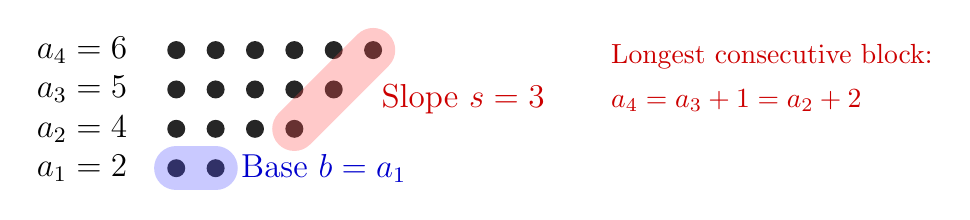
\begin{tikzpicture}[
	scale=0.5,
	dot/.style={circle, fill=black!85, minimum size=6.5pt, inner sep=0pt},
	highlight base/.style={blue!70, line width=16pt, opacity=0.3, line cap=round},
	highlight slope/.style={red!70, line width=16pt, opacity=0.3, line cap=round}
	]
	% Draw dots and row labels corresponding to the elements of S
	\foreach \y/\n/\label in {4/6/a_4, 3/5/a_3, 2/4/a_2, 1/2/a_1} {
		% Draw row label
		\node[left, font=\large] at (0, \y) {$\label = \n$};
		
		% Draw dots
		\foreach \x in {1,...,\n} {
			\node[dot] at (\x, \y) {};
		}
	}
	
	% Highlight Base
	\draw[highlight base] (1,1) -- (2,1);
	\node[blue!80!black, right, font=\large] at (2.4, 1) {Base $b = a_1$};
	
	% Highlight Slope
	\draw[highlight slope] (6,4) -- (4,2);
	
	% Brace for Slope
	\draw[decorate, decoration={brace, amplitude=8pt}, thick, white, shift={(.5,0)}, opacity=0] 
	(6.5, 4.5) -- (3, 1) 
	node[midway, right=10pt, align=left, font=\large, red!80!black,opacity=1] {Slope $s = 3$};
	
	% Text for slope definition
	\node[anchor=west, red!80!black, align=left] at (11.8, 3.3) {
		Longest consecutive block:\\[4pt]
		$a_4 = a_3+1 = a_2+2$
	};
\end{tikzpicture}
\end{center}
$b=2$ and $s=3$. 
We now define a map $\phi$ .
%on $S\subseteq\mathbb N$ with $\abs{S}<\infty$.
%\[
%\phi(S)=
%\begin{cases}
%	\{a_2,\dots,a_{r-b},\,a_{r-b+1}+1,\dots,a_r+1\}, & \text{if } b\le s,\\[1ex]
%	\{a_1,\dots,a_{r-s},\,a_{r-s+1}-1,\dots,a_r-1,\,s\}, & \text{if } b>s,
%\end{cases}
%\]
%where $S=\{a_1<\cdots<a_r\}$, $b=a_1$, and $s$ is the length of the longest consecutive block at the top of $S$.

%Let
%\[
%\mathcal F:=\{S\subseteq \mathbb N:\#S<\infty\}
%\]
%be the set of all finite subsets of $\mathbb N$.
%
%For a nonempty set
%\[
%S=\{a_1<a_2<\cdots<a_r\}\in\mathcal F,
%\]
%define its \emph{base} by
%\[
%b(S):=a_1,
%\]
%and define its \emph{slope} by
%\[
%s(S):=\max\{t\in\{1,\dots,r\}: a_r,a_{r-1},\dots,a_{r-t+1}
%\text{ are consecutive integers}\}.
%\]
%
%Define the exceptional set
%\[
%\mathcal E
%:=
%\Bigl\{\{k,k+1,\dots,2k-1\}:k\ge1\Bigr\}
%\cup
%\Bigl\{\{k+1,k+2,\dots,2k\}:k\ge1\Bigr\}.
%\]
%
%We define
%\[
%\phi:\mathcal F\setminus(\mathcal E\cup\{\varnothing\})\to \mathcal F
%\]
%as follows. Let
%\[
%S=\{a_1<a_2<\cdots<a_r\}\in \mathcal F\setminus(\mathcal E\cup\{\varnothing\}),
%\]
%and write
%\[
%b:=b(S),\qquad s:=s(S).
%\]
%
%\begin{itemize}
%	\item If $b\le s$, define
%	\[
%	\phi(S)
%	:=
%	\{a_2,\dots,a_{r-b},\,a_{r-b+1}+1,\dots,a_r+1\}.
%	\]
%	Equivalently, $\phi(S)$ is obtained by removing the smallest element $b$ and adding $1$ to each of the $b$ largest elements of $S$.
%	
%	\item If $b>s$, define
%	\[
%	\phi(S)
%	:=
%	\{a_1,\dots,a_{r-s},\,a_{r-s+1}-1,\dots,a_r-1,\,s\}.
%	\]
%	Equivalently, $\phi(S)$ is obtained by subtracting $1$ from each of the $s$ largest elements of $S$ and adjoining the element $s$.
%\end{itemize}

%\newpage
%We define a map
%\[
%\phi:\mathcal F\setminus\mathcal E\to \mathcal F\setminus\mathcal E,
%\]
%where $\mathcal F$ is the set of all finite subsets of $\mathbb N$, and $\mathcal E$ is the exceptional set.
%Define $\phi(S)$ by removing the smallest element $b$ and adding $1$ to each of the $b$ largest elements:
%\[
%\phi(S)
%=
%\{a_2,\dots,a_{r-b},\,a_{r-b+1}+1,\dots,a_r+1\}.
%\]
%Define $\phi(S)$ by subtracting $1$ from each of the $s$ largest elements and adjoining the element $s$:
%\[
%\phi(S)
%=
%\{a_1,\dots,a_{r-s},\,a_{r-s+1}-1,\dots,a_r-1,\,s\}.
%\]

\medskip

\noindent
\textbf{Case 1: $b< s$.}
Remove the smallest element $b$, and add $1$ to each of the $b$ largest elements.

\medskip

For example, if $S = \{a_1 < a_2 < a_3 < a_4\} = \{2, 4, 5, 6\}$, then $b=2$ and $s=3$.

\begin{center}
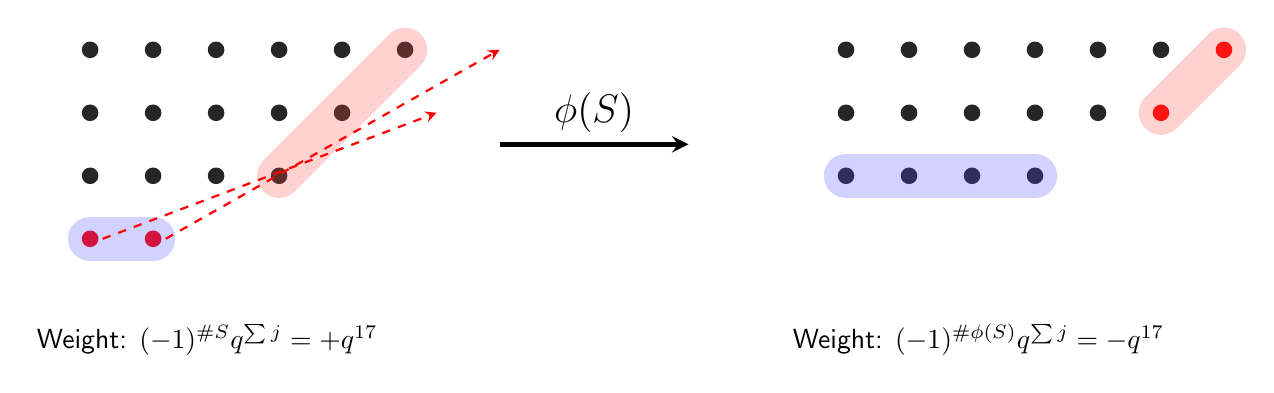
\begin{tikzpicture}[
	scale=0.8,
	dot/.style={circle, fill=black!85, minimum size=6pt, inner sep=0pt},
	movedot/.style={circle, fill=red, minimum size=6pt, inner sep=0pt},
	movearrow/.style={dashed, red, thick, ->, >=stealth, bend left=25},
	highlight base/.style={blue!70, line width=16pt, opacity=0.25, line cap=round},
	highlight slope/.style={red!70, line width=16pt, opacity=0.25, line cap=round}
	]
	
	% =========================================================
	% CASE 1: b <= s (Move Base to Slope)
	% Example: S = {2, 4, 5, 6}. b = 2, s = 3. b <= s.
	% =========================================================
	
	% --- Left Side: S ---
	\begin{scope}[xshift=0cm, yshift=4cm]
		% Draw static dots
		\foreach \y/\n in {4/6, 3/5, 2/4} {
			\foreach \x in {1,...,\n} {
				\node[dot] at (\x, \y) {};
			}
		}
		% Draw moved dots (the base)
		\node[movedot] (b1) at (1, 1) {};
		\node[movedot] (b2) at (2, 1) {};
		
		% Highlights
		\draw[highlight base] (1, 1) -- (2, 1);
		\draw[highlight slope] (6, 4) -- (4, 2);
		
		% Weight Annotation
		\node[anchor=north west, font=\sffamily, align=left] at (0, -0.2) {
%			$\sum_{j \in S} j = 6+5+4+2 = \mathbf{17}$\\[4pt]
%			$\#S = 4$ (Even)\\[4pt]
			Weight: $(-1)^{\#S} q^{\sum j} = +q^{17}$
		};
	\end{scope}
	
	% --- Mapping Arrow (phi) ---
	\draw[->, ultra thick, >=stealth] (7.5, 6.5) -- (10.5, 6.5) node[midway, above, font=\Large] {$\phi(S)$};
	% Curved arrows showing dot movement
	\draw[movearrow] (2.2, 5) -- (7.5, 8); % b2 to new s position 2
	\draw[movearrow] (1.2, 5) -- (6.5, 7); % b1 to new s position 1
	
	% --- Right Side: \phi(S) ---
	\begin{scope}[xshift=12cm, yshift=4cm]		
		% Draw static dots (same as left, y=1 row removed)
		\foreach \y/\n in {4/6, 3/5, 2/4} {
			\foreach \x in {1,...,\n} {
				\node[dot] at (\x, \y) {};
			}
		}
		% Draw newly arrived dots (added to the slope)
		\node[movedot] (s1) at (7, 4) {};
		\node[movedot] (s2) at (6, 3) {};
		
		% Highlights
		\draw[highlight base] (1, 2) -- (4, 2);
		\draw[highlight slope] (7, 4) -- (6, 3);
		
		% Weight Annotation
		\node[anchor=north west, font=\sffamily, align=left] at (0, -0.2) {
%			$\sum_{j \in \phi(S)} j = 7+6+4 = \mathbf{17}$\\[4pt]
%			$\#\phi(S) = 3$ (Odd)\\[4pt]
			Weight: $(-1)^{\#\phi(S)} q^{\sum j} = -q^{17}$
		};
	\end{scope}
\end{tikzpicture}
\end{center}
Then $\phi(S) = \{4, 6, 7\}$

\medskip

\noindent
\textbf{Case 2: $b>s$.}
Subtract $1$ from each of the $s$ largest elements, and adjoin the element $s$.

\medskip

For example, if $S' = \{a_1 < a_2 < a_34\} = \{4, 5, 7\}$, then $b=4$ and $s=2$.

\begin{center}
	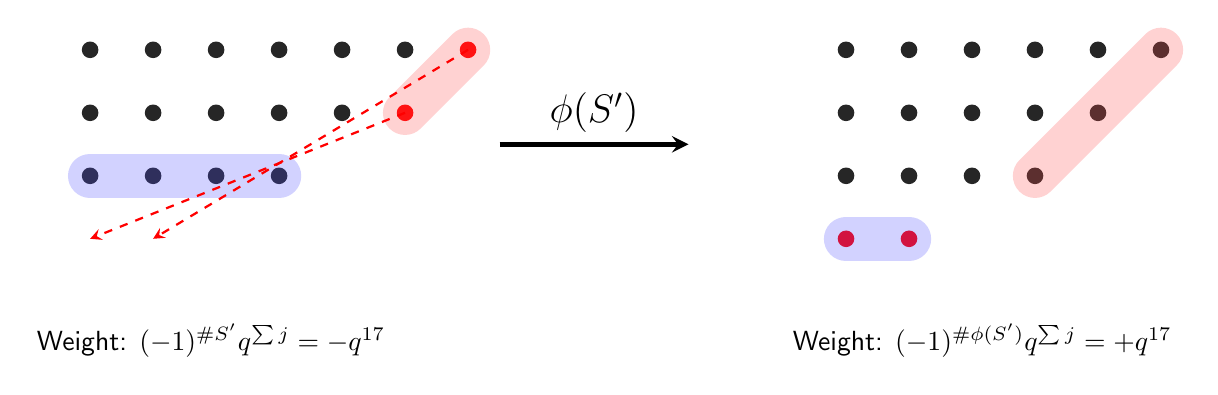
\begin{tikzpicture}[
	scale=0.8,
	dot/.style={circle, fill=black!85, minimum size=6pt, inner sep=0pt},
	movedot/.style={circle, fill=red, minimum size=6pt, inner sep=0pt},
	movearrow/.style={dashed, red, thick, ->, >=stealth, bend left=25},
	highlight base/.style={blue!70, line width=16pt, opacity=0.25, line cap=round},
	highlight slope/.style={red!70, line width=16pt, opacity=0.25, line cap=round}
	]
	% =========================================================
	% CASE 2: b > s (Move Slope to Base)
	% Example: S' = {4, 6, 7}. b = 4, s = 2. b > s.
	% =========================================================
	% --- Left Side: S' ---
	\begin{scope}[xshift=0cm, yshift=-8cm]
		% Draw static dots
		\foreach \y/\n in {4/6, 3/5, 2/4} {
			\foreach \x in {1,...,\n} {
				\node[dot] at (\x, \y) {};
			}
		}
		% Draw moved dots (the slope)
		\node[movedot] (sm1) at (7, 4) {};
		\node[movedot] (sm2) at (6, 3) {};
		
		% Highlights
		\draw[highlight base] (1, 2) -- (4, 2);
		\draw[highlight slope] (7, 4) -- (6, 3);
		
		% Weight Annotation
		\node[anchor=north west, font=\sffamily, align=left] at (0, -0.2) {
%			Sum = $\mathbf{17}$\\[4pt]
%			Elements = $3$ (Odd)\\[4pt]
			Weight: $(-1)^{\#S'} q^{\sum j} =-q^{17}$
		};
	\end{scope}
	
	% --- Mapping Arrow (phi inverse) ---
	\draw[->, ultra thick, >=stealth] (7.5, -5.5) -- (10.5, -5.5) node[midway, above, font=\Large] {$\phi(S')$};
	% Curved arrows showing dot movement
	\draw[movearrow] (7, -4) -- (2, -7); % sm1 to new b position 2
	\draw[movearrow] (6, -5) -- (1, -7); % sm2 to new b position 1
	
	% --- Right Side: S'' (Inverse mapped result) ---
	\begin{scope}[xshift=12cm, yshift=-8cm]
		% Draw static dots (same as above)
		\foreach \y/\n in {4/6, 3/5, 2/4} {
			\foreach \x in {1,...,\n} {
				\node[dot] at (\x, \y) {};
			}
		}
		% Draw newly arrived dots (forming the new base element s)
		\node[movedot] (b1_end) at (1, 1) {};
		\node[movedot] (b2_end) at (2, 1) {};
		
		% Highlights
		\draw[highlight base] (1, 1) -- (2, 1);
		\draw[highlight slope] (6, 4) -- (4, 2);
		
		% Weight Annotation
		\node[anchor=north west, font=\sffamily, align=left] at (0, -0.2) {
%			Sum = $\mathbf{17}$\\[4pt]
%			Elements = $4$ (Even)\\[4pt]
			Weight: $(-1)^{\#\phi(S')} q^{\sum j} = +q^{17}$
		};
	\end{scope}
\end{tikzpicture}
\end{center}
Then $\phi(S) = \{2,4,5,6\}$.

\medskip

By construction, $\sum_{j\in\phi(S)}j=\sum_{j\in S}j$.
%since in Case 1 we remove $b$ and add $1$ exactly $b$ times, while in Case 2 we subtract $1$ exactly $s$ times and then add $s$.
Moreover, \[
\#\phi(S)=\begin{cases}
\#S-1 &\text{if } b< s \\
\#S+1 &\text{if } b> s
\end{cases}
\]
Hence
\[
(-1)^{\#\phi(S)}q^{\sum_{j\in\phi(S)}j}
= \begin{cases}
	(-1)^{-1}(-1)^{\#S}q^{\sum_{j\in\phi(S)}j} &\text{if } b< s \\
	(-1)^{+1}(-1)^{\#S}q^{\sum_{j\in\phi(S)}j} &\text{if } b> s
\end{cases}=
-\,(-1)^{\#S}q^{\sum_{j\in S}j}.
\]

\newpage\noindent
The only subsets for which $\phi$ is not defined are the exceptional ones:
%\[
%\{k,k+1,\dots,2k-1\}
%\qquad\text{and}\qquad
%\{k+1,k+2,\dots,2k\},
%\qquad k\ge 1,
%\]
%together with the empty set.
\begin{enumerate}[(i)]
	\item ($b=s$)\; Let $S=\{k,k+1,\dots,2k-1\}$ ($k\geq 1$). For example, let $S = \{3, 4, 5\}$.  \begin{center}
		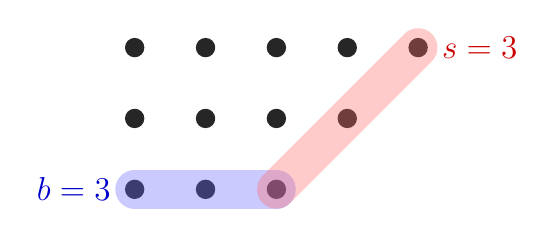
\begin{tikzpicture}[
		scale=0.9,
		dot/.style={circle, fill=black!85, minimum size=7pt, inner sep=0pt},
		base hl/.style={blue!60, line width=14pt, opacity=0.35, line cap=round},
		slope hl/.style={red!60, line width=14pt, opacity=0.35, line cap=round},
		panel frame/.style={draw=black!80, thick, rounded corners=4pt},
		panel title/.style={fill=black!5, text width=7.5cm, align=center, font=\sffamily\large\bfseries, inner sep=6pt, rounded corners=4pt},
		math text/.style={font=\large},
		desc text/.style={font=\sffamily, align=center, text width=7cm}
		]
		
		% =========================================================
		% Panel 1: Case 1 (b = s)
		% =========================================================
		\begin{scope}[xshift=0cm]
			% Dot Diagram (Centered roughly around x=4)
			\begin{scope}[xshift=1.5cm, yshift=4cm]
				\foreach \y/\n in {3/5, 2/4, 1/3} {
					\foreach \x in {1,...,\n} {
						\node[dot] at (\x, \y) {};
					}
				}
				% Highlights
				\draw[base hl] (1,1) -- (3,1);
				\draw[slope hl] (5,3) -- (3,1);
				
				% Labels
				\node[blue!80!black, left, font=\large] at (0.8, 1) {$b=3$};
				\node[red!80!black, right, font=\large] at (5.2, 3) {$s=3$};
			\end{scope}
		\end{scope}
	\end{tikzpicture}
	\end{center}
	The Base and Slope intersect at the exact same element. 
%	Removing $b$ and moving $s$ simultaneously is impossible.
	Since \[
	k+(k+1)+\cdots+(2k-1)
	=
	\frac{k}{2}\cdot(3k-1),\quad\text{and}\quad
	\#\{k,k+1,\dots,\underbrace{2k-1}_{=k+(k-1)}\}=k,
	\] we have \[
	\boxed{(-1)^{\#S}q^{\sum_{j\in S}j}=(-1)^k q^{k(3k-1)/2}.}
	\]
	\item ($b=s+1$)\; Let $S=\{k+1,k+2,\dots,2k\}$ ($k\geq 1$). For example, let $S = \{4, 5, 6\}$.
	\begin{center}
		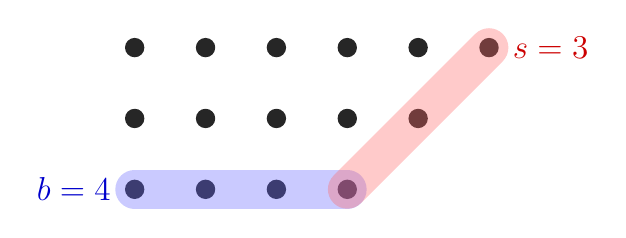
\begin{tikzpicture}[
			scale=0.9,
			dot/.style={circle, fill=black!85, minimum size=7pt, inner sep=0pt},
			base hl/.style={blue!60, line width=14pt, opacity=0.35, line cap=round},
			slope hl/.style={red!60, line width=14pt, opacity=0.35, line cap=round},
			panel frame/.style={draw=black!80, thick, rounded corners=4pt},
			panel title/.style={fill=black!5, text width=7.5cm, align=center, font=\sffamily\large\bfseries, inner sep=6pt, rounded corners=4pt},
			math text/.style={font=\large},
			desc text/.style={font=\sffamily, align=center, text width=7cm}
			]
	% =========================================================
	% Panel 2: Case 2 (b = s + 1)
	% =========================================================
	\begin{scope}[xshift=8.5cm]
		% Dot Diagram (Centered roughly around x=4)
		\begin{scope}[xshift=1cm, yshift=4cm]
			\foreach \y/\n in {3/6, 2/5, 1/4} {
				\foreach \x in {1,...,\n} {
					\node[dot] at (\x, \y) {};
				}
			}
			% Highlights
			\draw[base hl] (1,1) -- (4,1);
			\draw[slope hl] (6,3) -- (4,1);
			
			% Labels
			\node[blue!80!black, left, font=\large] at (0.8, 1) {$b=4$};
			\node[red!80!black, right, font=\large] at (6.2, 3) {$s=3$};
		\end{scope}
	\end{scope}
	\end{tikzpicture}
	\end{center}
	The Base and Slope intersect. Since \[
	(k+1)+(k+2)+\cdots+2k
	=
	\frac{k}{2}\cdot(3k+1),\quad\text{and}\quad
	\#\{k+1,k+2,\dots,\underbrace{2k}_{=k+k}\}=k,
	\] we obtain \[
	\boxed{(-1)^{\#S}q^{\sum_{j\in S}j}=(-1)^k q^{k(3k+1)/2}}.
	\]
	\item ($S=\varnothing$)\; The empty set has no elements, so it has neither a base $b$ nor a slope $s$. Then \[
	\boxed{(-1)^{\#\varnothing}q^{\sum_{j\in \varnothing}j}=(-1)^0q^0=1}.
	\]
\end{enumerate}
%Therefore
%\[
%\sum_{\substack{S\subseteq\mathbb N,\ \#S<\infty}}
%(-1)^{\#S}q^{\sum_{j\in S}j}
%=
%1+\sum_{k=1}^\infty (-1)^k q^{k(3k-1)/2}
%+\sum_{k=1}^\infty (-1)^k q^{k(3k+1)/2}.
%\]
Hence
\begin{align*}
\prod_{j=1}^\infty(1-q^j)=\lim_{N\to\infty}\prod_{j=1}^N(1-q^j)
&=\lim_{N\to\infty}\sum_{S\in\mathcal P_N}(-1)^{\#S}q^{\sum_{j\in S}j}\\
	&=1+\sum_{k=1}^\infty (-1)^k q^{k(3k-1)/2}+\sum_{k=1}^\infty (-1)^k q^{k(3k+1)/2}\\
	&=\underbrace{(-1)^0q^0}_{k=0}+\sum_{k=1}^\infty (-1)^{k} q^{k(3k-1)/2}+
	\sum_{k=-\infty}^{-1} (-1)^{-k} q^{{-k}(3(-k)+1)/2}\\
	&=\sum_{k=-\infty}^{-1} (-1)^{k} q^{{k}(3k-1)/2}+
	{(-1)^0q^0}+\sum_{k=1}^\infty (-1)^{k} q^{k(3k-1)/2}\\
	&=\sum_{k=-\infty}^{\infty}(-1)^k q^{k(3k-1)/2}.
\end{align*}
\end{proof}

%\newpage
%\begin{notation}
%We define the \textbf{ring of formal power series} in $x$ with integer coefficients \[
%\mathbb{Z}[[x]]:=\left\{\sum_{n=0}^\infty a_nx^n:a_n\in\Z\right\}.
%\]
%(Operation)\; For $f(x)=\sum_{n=0}^\infty a_nx^n,\; g(x)=\sum_{n=0}^\infty b_nx^n$, define
%\[
%f(x)+g(x)=\sum_{n=0}^\infty (a_n+b_n)x^n\qquad\text{and}\qquad
%f(x)g(x)=\sum_{n=0}^\infty c_nx^n,
%\quad
%c_n=\sum_{k=0}^n a_kb_{n-k}.
%\]
%(Identity)\; In $\Z[[x]]$, the \textbf{additive identity} is the zero series \[
%0=0+0x+0x^2+\cdots=\sum_{n=0}^\infty0x^n,
%\] and the \textbf{multiplicative identity} is \[
%1=1+0x+0x^2+\cdots=\sum_{n=0}^\infty c_nx^n\quad\text{with}\quad c_n=\begin{cases}
%	1 &\text{if } n = 0\\
%	0 &\text{if } n\geq 1
%\end{cases}.
%\]
%%Since each $c_n$ is a finite sum of integers, $c_n\in\mathbb{Z}$, so $f(x)g(x)\in\mathbb{Z}[[x]]$.
%%Thus $\mathbb{Z}[[x]]$ is a commutative ring with identity.
%\end{notation}

\begin{tcolorbox}[colback=white, colframe=axiomcolor,title={\textbf{Pentagonal Number Theorem}}]
\begin{theorem}
%In the ring $\mathbb{Z}[[x]]$, one has 
%\[
%\prod_{j=1}^{\infty}(1-x^j)
%=
%1+\sum_{k=1}^{\infty}(-1)^k
%\left(x^{k(3k-1)/2}+x^{k(3k+1)/2}\right).
%\] 
%Equivalently,
%\[
%\prod_{j=1}^{\infty}(1-x^j) =
%\sum_{k=-\infty}^{\infty}(-1)^k x^{k(3k-1)/2}.
%\]
%It converges for $\abs{x}<1$.
%If $|x|<1$, then
%\[
%1+\sum_{k=1}^{\infty}(-1)^k
%\left(x^{k(3k-1)/2}+x^{k(3k+1)/2}\right)
%\]
%and
%\[
%\sum_{k=-\infty}^{\infty}(-1)^k x^{k(3k-1)/2}
%\]
%both converge absolutely. Moreover,
%\[
%\prod_{j=1}^\infty(1-x^j)=1+\sum_{k=1}^{\infty}(-1)^k
%\left(x^{k(3k-1)/2}+x^{k(3k+1)/2}\right)
%=
%\sum_{k=-\infty}^{\infty}(-1)^k x^{k(3k-1)/2}.
%\]
The series \begin{align*}
\prod_{j=1}^\infty(1-x^j)
&=1+\sum_{k=1}^{\infty}(-1)^k
\left(x^{k(3k-1)/2}+x^{k(3k+1)/2}\right)\\
&=\sum_{k=-\infty}^{\infty}(-1)^k x^{k(3k-1)/2}.
\end{align*} converge for \(|x|<1\)
\end{theorem}
\end{tcolorbox}
\begin{proof}
Note that \[
\sum\abs{a_n}<\infty\implies\sum a_n\text{ converges.}
\] We want to prove that the series \[
1+\sum_{k=1}^{\infty}(-1)^k
\left(x^{k(3k-1)/2}+x^{k(3k+1)/2}\right)\quad\text{converges absolutely when $|x|<1$. }
\]
Indeed,
\[
\sum_{k=1}^{\infty}
\left|x^{k(3k-1)/2}+x^{k(3k+1)/2}\right|
\le
\sum_{k=1}^{\infty}
\left(|x|^{k(3k-1)/2}+|x|^{k(3k+1)/2}\right).
\]
Since for every \(k\ge 1\), \[
\frac{k(3k-1)}2\ge k,
\qquad
\frac{k(3k+1)}2\ge k\qquad\implies\qquad
|x|^{k(3k-1)/2}\le |x|^k,
\qquad
|x|^{k(3k+1)/2}\le |x|^k.
\]
Therefore
\[
\sum_{k=1}^{\infty}
\left(|x|^{k(3k-1)/2}+|x|^{k(3k+1)/2}\right)
\le
2\sum_{k=1}^{\infty}|x|^k.
\]
The geometric series on the right converges because \(|x|<1\). Hence
\[
1+\sum_{k=1}^{\infty}(-1)^k
\left(x^{k(3k-1)/2}+x^{k(3k+1)/2}\right)\quad\text{
	converges absolutely for $|x|<1$.}
\]
\end{proof}
%\begin{remark}
%The exponents $\displaystyle\frac{k(3k\pm1)}{2}\; (k\ge 1)$
%are called the \emph{generalized pentagonal numbers}.
%\end{remark}


\begin{tcolorbox}[colback=white, colframe=axiomcolor,title={\textbf{Pentagonal Number Theorem}}]
\begin{theorem}
Let $n\geq 2$. Then \[
\Pr[\textbf{M}\xleftarrow{\$}\mathrm{Mat}_{n}(\F_2):\det(\textbf{M})\neq 0] > 0.288788.
\]
\end{theorem}
\end{tcolorbox}

\begin{proof}
%Recall that \[
%|\Mat_n(\F_q)|=q^{n^2},
%\qquad
%|GL_n(\F_q)|=\prod_{i=0}^{n-1}(q^n-q^i),
%\]
%and hence \begin{align*}
%	\frac{|GL_n(\F_q)|}{|\Mat_n(\F_q)|} =
%	\frac{\prod_{i=0}^{n-1}(q^n-q^i)}{q^{n^2}}
%	&= \frac{1}{q^{n^2}}\left[(q^n-1)(q^n-q)(q^n-q^2)\cdots(q^n-q^{n-1})\right] \\
%	&= \frac{1}{q^{n^2}}\left[q^n\Bigg(1-\frac{1}{q^n}\Bigg)\Bigg(1-\frac{1}{q^{n-1}}\Bigg)\Bigg(1-\frac{1}{q^{n-2}}\Bigg)\cdots\Bigg(1-\frac{1}{q^{1}}\Bigg)\right]\\
%	&= \Bigg(1-\frac{1}{q^n}\Bigg)\Bigg(1-\frac{1}{q^{n-1}}\Bigg)\Bigg(1-\frac{1}{q^{n-2}}\Bigg)\cdots\Bigg(1-\frac{1}{q^{1}}\Bigg)\\
%	&=\prod_{j=1}^{n}(1-q^{-j}).
%\end{align*}
Define
\[
P_n:=\prod_{j=1}^n(1-2^{-j})
\]
Since $P_n$ is a decreasing sequence, we have \[
P_n>\prod_{j=1}^\infty(1-2^{-j})\quad\text{for every $n\ge 2$. }
\] Applying pentagonal-number theorem, we obtain
\[
\prod_{j=1}^\infty(1-2^{-j})=
1+\sum_{k=1}^\infty (-1)^k\left(2^{-k(3k-1)/2}+2^{-k(3k+1)/2}\right).
\]
Therefore \begin{align*}
\prod_{j=1}^\infty(1-2^{-j})
&=
1-\left(2^{-1}+2^{-2}\right)
+\left(2^{-5}+2^{-7}\right)
-\left(2^{-12}+2^{-15}\right)
+\left(2^{-22}+2^{-26}\right)-\cdots\\
&>
1-\left(2^{-1}+2^{-2}\right)
+\left(2^{-5}+2^{-7}\right)
-\left(2^{-12}+2^{-15}\right)
+2^{-22}\\
&=1-\frac12-\frac14+\frac1{32}+\frac1{128}-\frac1{4096}-\frac1{32768}+\frac1{4194304}\\
&=0.2887880802154541\ldots \\
&> 0.288788.
\end{align*}
Since \(P_n>\prod_{j=1}^\infty(1-2^{-j})\), it follows that
\[
\Pr[\mathbf M\xleftarrow{\$}\Mat_n(\F_2):\det(\mathbf M)\neq 0]
=\prod_{j=1}^n(1-2^{-j})
>0.288788.
\]
\end{proof}

\medskip

\begin{center}
\begin{minipage}{.475\textwidth}
\begin{lstlisting}[style=sagemath, numbers=none]
def pentagonal_series(N):
	R = RealField(50)
	return R(1) + sum(
		(-1)^k * (R(2)^(-k*(3*k-1)/2) 
		+ R(2)^(-k*(3*k+1)/2))
		for k in range(1, N+1)
	)

for r in range(1, 11):
	s = pentagonal_series(r)
	print(f"(1 to {r+1:2d}) partial sum = {s}")
\end{lstlisting}
\begin{lstlisting}
(1 to  2) partial sum = 0.25000000000000
(1 to  3) partial sum = 0.28906250000000
(1 to  4) partial sum = 0.28878784179688
(1 to  5) partial sum = 0.28878809511662
(1 to  6) partial sum = 0.28878809508660
(1 to  7) partial sum = 0.28878809508660
(1 to  8) partial sum = 0.28878809508660
(1 to  9) partial sum = 0.28878809508660
(1 to 10) partial sum = 0.28878809508660
(1 to 11) partial sum = 0.28878809508660
\end{lstlisting}
\end{minipage}\hfill
\begin{minipage}{.475\textwidth}
\begin{lstlisting}[style=sagemath, numbers=none]
def bilateral_pentagonal_series(N):
	R = RealField(50)
	return sum(
		(-1)^k * R(2)^(-k*(3*k-1)/2) 
		for k in range(-N, N+1)
	)

for r in range(1, 11):
	s = bilateral_pentagonal_series(r)
	print(f"(-{r:2d} to {r+1:2d}) partial sum = {s}")
\end{lstlisting}
\begin{lstlisting}
(- 1 to  2) partial sum = 0.25000000000000
(- 2 to  3) partial sum = 0.28906250000000
(- 3 to  4) partial sum = 0.28878784179688
(- 4 to  5) partial sum = 0.28878809511662
(- 5 to  6) partial sum = 0.28878809508660
(- 6 to  7) partial sum = 0.28878809508660
(- 7 to  8) partial sum = 0.28878809508660
(- 8 to  9) partial sum = 0.28878809508660
(- 9 to 10) partial sum = 0.28878809508660
(-10 to 11) partial sum = 0.28878809508660
\end{lstlisting}
\end{minipage}
\end{center}


%\vfill
%\footer{Departnent of Cyber Security\\ [4pt]
	%%	College of Science and Technology\\
	%	Kooknin University}
\end{document}